\documentclass{article}

% if you need to pass options to natbib, use, e.g.:
% \PassOptionsToPackage{numbers, compress}{natbib}
% before loading nips_2016
%
% to avoid loading the natbib package, add option nonatbib:
% \usepackage[nonatbib]{nips_2016}

\usepackage{nips_2016}

% to compile a camera-ready version, add the [final] option, e.g.:
% \usepackage[final]{nips_2016}

\usepackage[utf8]{inputenc} % allow utf-8 input
\usepackage[T1]{fontenc}    % use 8-bit T1 fonts
\usepackage{hyperref}       % hyperlinks
\usepackage{url}            % simple URL typesetting
\usepackage{booktabs}       % professional-quality tables
\usepackage{amsfonts}       % blackboard math symbols
\usepackage{nicefrac}       % compact symbols for 1/2, etc.
\usepackage{microtype}      % microtypography
\usepackage[final]{graphicx}

\title{Accuracy of secondary protein structure prediction tools for chromoproteins and fluorescent proteins}

\begin{document}
% \nipsfinalcopy is no longer used

 Rachael C.~Kretsch \\
 Mathematics of Big Data, Fall 2016\\
 Harvey Mudd College\\
 \texttt{rkretsch@g.hmc.edu} \\

\maketitle

\begin{abstract}
   Secondary protein prediction is a useful tool for a first investigation of a new protein. Methods have been developed since the 1970s to accurately predict the secondary structure, however, these methods attempt to generalize to the large majority of proteins, thus ignoring special patterns in special classes of proteins. This is especially true of new methods that focus on predicting disordered coils due to their difficultly to see experimentally, but this also biases the predictor towards predicting coils. Chromoproteins and florescent proteins are of vital importance to biological experimentation, however, they are very structured, and therefore predictors are poor at predicting its secondary structure. By learning the structure of these proteins we can target the color producing areas for mutation so that we can change the function. To do so, I develop a logistic regression model, fit specifically on these proteins, to attempt to provide a model that can accurately predict their structure. Although my method outperformed some older methods from the 1990s, SOPM and GORIV, a modern method, sD2, predicted the sequences more accurately despite a 20\% reduction in its average accuracy. It may be interesting to use these modern methods trained on a biased data set to see if this provides a better predictor.
\end{abstract}

\section{Introduction}

\subsection{Secondary protein structure prediction}

This project aims to look at methods to predict secondary protein structure. Protein structure prediction is a major field of study and is a problem that takes massive computational power to solve. There are two main approaches looking from a biochemical point of view. The first is isolated the protein, crystallizing it, and performing crystal chromatography to figure out the structure. This structure is relaxed into its hypothesized structure via molecular dynamics. The second method is experimentally less intense. One of the most plentiful and easy to obtain biological data is DNA sequence. From the DNA sequence of a coding region there are simply rules to propose a great starting point for the protein's amino acid sequence. The problem of predicting the 3D structure from an amino acid sequence is extremely hard. I will reduce this problem to simpler features. My aim is to look at how we can use the amino acid sequence, the primary structure, to deduce secondary structure components like $\beta$-sheets, $\alpha$-helices, and coils. 

The field of computationally predicting secondary structures has been active since the 1970s [7]. The large majority of these methods are extremely generalizable to proteins of all classes. The training databases used for these methods are often very diverse with a goal of less than 25(\%) homology between each protein [8]. This projects inspiration drew from a method created by Cambria, called Hydropathy Clustering Assisted Methods [3]. This method is specifically designed to give accurate prediction for water soluble globular proteins, which are often difficult to predict using the conventional generalizable methods because of their special hydrophobicity concerns. This project concerns itself with a group of proteins, chromoproteins and florescent proteins, whose secondary structure is predicted with below average accuracy using traditional methods, however, their secondary structure is an excellent indicator for identifying important parts of the protein for manipulation.

\subsection{Fluorescent proteins and chromoproteins}
Chromoproteins and fluorescent proteins are vital for biological and medical research. Chromoproteins are colored proteins and fluorescent proteins fluoresce light when they absorb a certain wavelength. They are used to target and visualize components of interest. As biological research progresses, proteins with more extreme properties such as new colors, and fluorescence able to pass through thick skin are needed. Finding these in nature is very difficult so the best method is to mutate current proteins and increase their functionality. The structure of these chromoproteins and fluorescent proteins is very important and quite conserved between proteins. The structures are mostly $\beta$-strands that wrap into $\beta$-barrels. Inside these barrels are coils that have been shown to be vital for the fluorescent properties of these proteins. Mutations to these coils cause dramatic changes in function from increasing function to changing wavelength of absorbtion. Obtaining structural data from experiment, either NMR or x-ray crystallography, can be very difficult and time consuming. On the other hand sequencing DNA is very simple, quick, and cheap. In fact the cost of sequencing is decreasing quicker than Moores law! Therefore, a computational method to convert sequence to structure would help experimentalists target areas for mutation. Because chromoproteins and fluorescent proteins have relatively predictable structural elements and these are almost wholly defined by secondary structure, they are excellent candidates for secondary protein structure predictions.


\section{Methods and materials}

\subsection{Logistic regression method implementation}

The protein sequences were extracted from the Protein Data Base [10] from results of the searches "chromoprotein" and "florescent". Proteins less than 25 amino acids in length were removed as well as any sequences with the same ID, the first sequence was kept. This left a dataset of 739 with a total of 392,106 amino acids. The correct secondary structure to which each amino acid in these sequences belong was extracted from DSSP [1],[2], a standardized database for interpretations of NMR and crystallography results. Scoring matrices were created by analyzing the frequency that each amino acid was part of each structure. $\alpha$-helices and 3-helices were identified as helical structures and were given a weight of 1. $\beta$-strands and $\beta$-bridges were identified as $\beta$ structures and were given a weight of -1. The remaining structures, 5-helices, turns, and bends were identified as coil structures and given a weight of 0. Essentially this model assumes that a amino acid is either in a correct environment to form a helical structure or a $\beta$ structure and if the preference for either is not strong enough, then is coils. The averaged score of an amino acid, was simply calculated by looking at all instances in the data set and averaging the described weights. This was also done for the neighboring amino acids up to 3 amino acids away. 3 was selected, because an helix can only form with 6 amino acids so we needed to be analyzing interactions at least 3 away to predict and helix. Matrices were created for each amino acid with the scores of itself and that neighbor scores for the surrounding 6 amino acids. This create a data set of 2,744,742 data points. A quarter of the data was randomly selected as a validation set. A multinomial logistic regression was performed on the remaining 75(\%) of the data. L2 regression was shown to be the most precise with a regularization factor of 3.4. Accuracy was calculated according the the convention of secondary structure prediction methods, Q3.

$$Q3=\sum_{n=1}^{k} NC(i)/NO(i) $$

where NC(i) is the number of correct amino acid predictions for protein i, and NO is the number of observed amino acids for protein i.

\subsection{Literature method testing}

\subsubsection{GORIV [4]}

GORIV is a secondary protein structure prediction method based in information theory and bayesian statistics. It uses the basis that given a data set os sufficient size we can find the probability of an amino acid of some type being a certain secondary structure. This can be extended to joint distributions involving the amino acids next door. The result in an expression for the probability of the confirmation S at a position i given the surrounding amino acid identities $R_n$

$$I(\Delta S_i ; R_1, ... , R_n) = log[\frac{P(S_i,R_1,...,R_n)}{P(n-S_i,R_1,...,R_n)}] + log[\frac{P(n-S)}{P(S)}]$$

Each version of GOR has made different approximations to this probability to simplify the calculation. The first couple of methods assumed that only the 8 neighboring amino acids would have a influence on the secondary structure, limiting the window to 17 amino acids. GOR III then included pairwise information. Essentially how the pair of amino acids affected the structure at each position. They also had to introduce dummy frequencies because their dataset was too small to have reliable results for the rare amino acids. In the GOR IV they increased the data base size so dummy frequencies were no longer necessary. The also increased the pairwise comparisons from just comparisons between the central amino acid to the others its window to comparisons between all amino acids in the window.

$$log[\frac{P(S_i,R_1,...,R_17)}{P(n-S_i,R_1,...,R_17)}] = \frac{2}{17}  \sum_{m=-8, n>m}^{+8}log[\frac{P(S_i,R_i+m,R_i+n)}{P(n-S_i,R_i+m,R_i+m}] $$
$$ -\frac{15}{17}  \sum_{m=-8}^{+8}log[\frac{P(S_i,R_i+m)}{P(n-S_i,R_i+m}]$$

The method has a training data base of 267 proteins. The newest update, GORV, included evolutionary data to increase accuracy, but GOR IV was used in this study [9].

The sequences prediction data was calculated from \url{https://npsa-prabi.ibcp.fr/cgi-bin/npsa_automat.pl?page=/NPSA/npsa_gor4.html}.

\subsubsection{SOPM [5]}

The first step for the SOPM method is to generate a limited database. This is done by using an alignment algorithm by Needleman and Wunsch (1970) [11] to pairwise compare the input protein to the proteins in the reference database. Because, this alignment method, as with most alignment methods, is parameterized with the idea that sequences compared will be quite similar we must be very careful because we are comparing proteins that are sometimes vastly different, especially in length. The parameter that is most volatile is the gap penalty, the parameter that penalizes a large insertion not present in the other sequences. To reduce this, 5 randomized copies of each protein of the reference database were created. The averaged randomized score was taken as the noise, and the actual protein sequence similarity could then be separated from this noise. The database is selected from the group of proteins most similar to the input protein. However, only one of each highly related protein is added so as not to skew the prediction parameters by a large group of very similar structures and sequences. 

The second and third step consist of a continuous loop until prediction accuracy is sufficient. Firstly, we loop through all the protein in the sub-database and individually predict their secondary structure using the data from the other proteins in the sub database. This is accomplished by breaking the protein into 17 overlapping amino acid sequences which are then compared. The scores are accumulated as each protein is compared. There are adjustment parameters for each of these scores representing the adjustment for $\alpha$-helix, $\beta$-sheet, and coils. These are optimized every step by the following equation

$$f_k(i+1) = f(i) + \frac{NO(i)-NP_k(i))}{NP_k(i)}$$

where NO(i) is the total amount of amino acids observed and $NP_k$ is the amount of amino acids predicted as k structured. When the fit is satisfactory it uses the fit to predict the input protein. The method has a training database of 239 proteins.

The sequences prediction data was calculated from \url{https://npsa-prabi.ibcp.fr/cgi-bin/npsa_automat.pl?page=npsa_sopm.html}. The sequence was predicted for the 3 structures, with a similarity threshold value of 8 and a window length of 17.

\subsubsection{s2D [8]}

This is the newest method tested and therefore predictably has the largest training set of 2671 proteins. This method, along with SPIDER, are the most promising secondary structure predictors. This method is of particular interest to this problem because of the development of the s2D dataset on which it was trained. The set was taken from the Biological Magnetic Resonance Bank which is a database of NMR spectroscopical data for proteins [12]. NMR is especially useful for disordered proteins which have a high concentration of coils. Therefore, their data set was only 18\% $\beta$-strands and was biased toward stable disordered forms of the protein. To correct this they looked for other data that had less than 25\% sequence matching with the database and more than 18\% $\beta$ residues. They reported that this increased the proportional $\beta$ strands by 83\%, however there is still the potential for bias which this data set of high $\beta$-barrel concentration will test. The data did show there was a higher false positive rate for coil structures, however $\beta$ structures were lower than helices in false positive rate [8].

This method first scores the data using position-specific scoring matrix from the PSI-BLAST program, a commonly used tool for multiple alignment [13]. This gave each amino acid 22 input values. The first step is two single hidden layer feedforward neural networks that are identical except that one has a window read of 11 amino acids and the other of 15 amino acids. They have output neurons representing the secondary-structure populations for the three secondary structures. It then uses an N-to-1 network to find the mean secondary structure populations of the whole protein, thus overcoming the problem of the proteins having variable lengths. The N-to-1 network uses the 22 original inputs as well as the 6 new inputs from the SLFNs. A final SLFN takes this output and uses a 5 amino acid window to look at neighboring amino acids and correct discrepancies. It also receives global data from the N-to-1 network which allows it to consider some stabilizing effects that are longer distance

The sequences prediction data was calculated from \url{http://www-mvsoftware.ch.cam.ac.uk/index.php/s2D}.

\subsection{Comparing methods}
The four methods were compared for the 20 amino acids that the logistic regression performed best and worst on. The accuracies were compared for each of these proteins. The identity, function, and structure was also manually analyzed to investigate if there were any patterns that caused a method to fail.


\section{Results}

\subsection{Logistic regression}

\begin{figure}[h]
  \centering
  \fbox{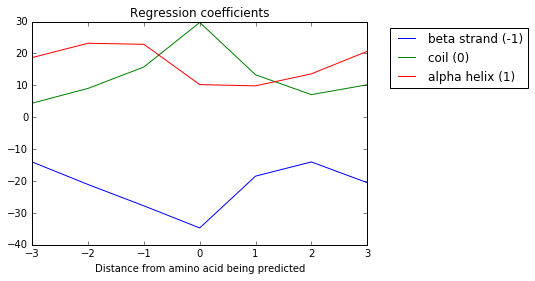
\includegraphics[width=\textwidth]{re_coef}}
  \caption{Logistic regression fit coefficients.}
\end{figure}

The logistic regression parameters were chosen to be L2 regression and a regression parameter of 3.4 after testing L1 regression and other regression parameters that yielded weaker results. The coefficients of the fit are seen in Figure 1. It is noteworthy that  helices are clearly disfavored in this fit, most likely because of their minimal presence in the data set, so the fit is skewed towards their improbability. Interestingly both $\beta$ structures are more strongly predicted by neighboring amino acids then its own. This is probably because all amino acids can form a $\beta$ structure (unlike helical structures) so it is more important that the environment is correct (alternating polar/non-polar residues) than the amino acid itself. The selection of the training set was shown to not have a significant effect on the accuracy. The accuracy of individual protein selection was skewed towards high accuracies and centered around 54(\%) (Figure 2).

\begin{figure}[h]
  \centering
  \fbox{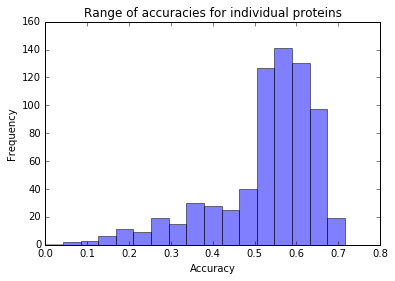
\includegraphics[width=\textwidth]{accuracies}}
  \caption{Range of accuracies in the data set. }
\end{figure}

\subsection{Method comparison}

\begin{table}[t]
  \caption{Accuracy of various secondary structure prediction methods}
  \centering
  \begin{tabular}{lll}
    \toprule
    Method     & Accuracy on data set (\%)    & Reported accuracy (\%)\\
    \midrule
    Logistic regression & 54 & -     \\
    GORIV     & 48 & 64      \\
    SOPM     & 51      & 69  \\
    s2D     & 64       & 85-88  \\
    \bottomrule
  \end{tabular}
\end{table}


All three literature methods tested had poorer accuracies for the chromoproteins and florescent proteins than the average accuracy value they report (table 1). This is likely because they are not trained specifically on such a $\beta$ rich data set. Interestingly, my logistic regression method was more accurate than both the GOR IV method and SOPM method. These methods utilized similar techniques to what I did and similar computational power. I believe that training on a very similar data set allowed my method to out perform these methods. s2D performed the best as expected, although it did perform an average of 20\% worse than its reported accuracies perhaps hinting at it's weakness at predicted the structures of highly organized $\beta$-barrel containing proteins.

\begin{table}[t]
  \caption{Accuracy of methods for specific proteins}
  \centering
  \begin{tabular}{lllll}
    \toprule
    \multicolumn{5}{c}{Accuracies (\%)}\\
    \cmidrule{2-5}
    Protein ID & Logistic regression & GORIV & SOPM & s2D\\
    \midrule
    1bgp & 25 & 64&62&64 \\
    4q7t & 25 & 44 & 42 & 67 \\
    4qgw & 25 & 69 & 61 & 83 \\
    5h88 & 26 & 37&37&57 \\
    4l1s & 26 & 64&52&70 \\
    
    5h89 & 27 & 37&39&60 \\
    3s0f & 27 & 49 & 58 & 70 \\
    4q9w & 27 & 51&55&70 \\
    3rwt & 27 & 37&35&48 \\
    5hzo & 28 & 37 & 46 & 64 \\
    \midrule
    1bfp & 60 & 48&60&77 \\
    3ekh & 60 & 54&61&55 \\
    3ned & 60 & 40&46&73 \\
    4k3g & 60 & 49&54&59 \\
    3cfc & 60 & 58 &60&61 \\
    
    1xkh & 60 & 50&48&47 \\
    2wht & 60 & 37&58&70 \\
    4w6b & 60 & 44&54&69 \\
    4xvp & 60 & 44&49&52 \\
    3dqh & 60 & 42&56&73 \\
    \bottomrule
  \end{tabular}
\end{table}

When analyzing the 10 proteins predicted best by the logistic regression method and the 10 proteins that were predicted worst we see a general pattern that the ones predicted best mostly had $\beta$-barrels while the ones predicted worst often had helices that was never predicted by this model. To look at a couple examples, the protein 3s0f performed very poorly in my method because is has a high concentration of helices. 3ekh and 3cfc structures were predicted well by my method, but not by not by the other methods especially s2D. This could be because they are highly concentrated in $\beta$ structures.

\begin{figure}[h]
  \centering
  \fbox{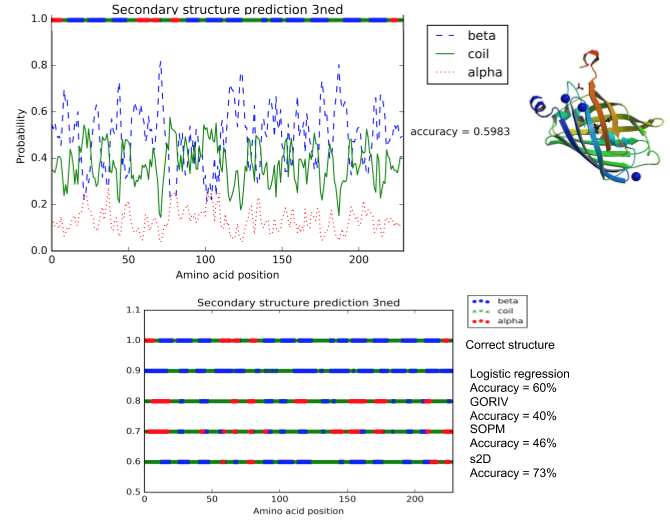
\includegraphics[width=\textwidth]{3ned}}
  \caption{Method comparison for 3ned. }
\end{figure}

3ned was a protein whose structure was predicted very well in the logistic regression model and the s2D model but not GOR IV or SOPM. We can see in figure 3 that it is a simple single $\beta$-barrel, this could indicated why the logistic regression trained on a $\beta$-barrel performed so well. This is a mutant of the mRounge florescent protein that had 16 mutations and increase red florescence. It was recently created with the aid of a computationally design library, essentially a program that directed the scientists were to mutate. Notice is figure 3 that GOR IV and SOPM over predicted helices while s2D and logistic regression both are biased against helices so did not have an issue. 

\begin{figure}[h]
  \centering
  \fbox{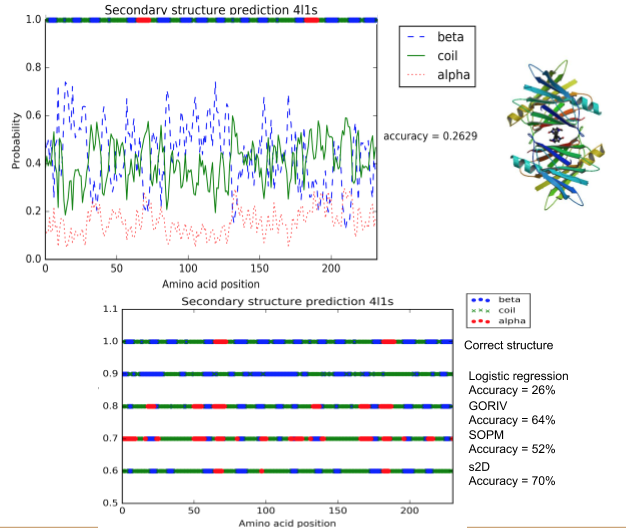
\includegraphics[width=\textwidth]{4l1s}}
  \caption{Method comparison for 4l1s. }
\end{figure}

4l1s is an interesting protein that performed very poorly in the logistic regression model, 26\% prediction accuracy, while the structure was predicted decently in the other methods. This is in fact a transport protein found inside the membrane, unlike most other florescent proteins, and only fluoresces when it is conjugated with another protein. These discrepancies from the typical protein this model was trained on explains its poor performance. This indicates that the logistic regression model does not generalize to other proteins as expected

\section{Discussion}

The method develop could be used on a chromoproteins or florescent protein whose structure is unknown. Let's say a new protein is discovered that has far-red florescence and we want to try and increase this function. We could use this method to predict were the coil structures are and pinpoint these parts of the sequence for mutations. This targeted approach would be a vast improvement over random mutations for experimental biologists.

Overall the logistic regression method performed well for proteins with the expected highly conserved structures. This is especially promising because a large amount of mutated proteins were predicted accurately which may allow for targeted modifications in the future. Despite this, neural network techniques, like s2D or perhaps SPIDER, are still stronger predicting models. Perhaps implementing these methods with biased sets could yield beneficial results.

The accuracy measurement could be adjusted to give a more precise picture. Each method gives the probability that the given amino acid is each secondary structure. So these confidence intervals could be used to improve the accuracy measurements.

More generalized methods need to be investigated to conclude that chromoproteins and florescent protein secondary structure is not accurately predicted by these and warrants another method. One such method is YASSP, which focuses on choosing optimal kernels in a cascaded model constructed from two SVM-based models [6]. Furthermore, it could be interesting to investigate changing training sets for these all these methods. These methods are trained on very varied data sets, most without data from mutants. It could be interesting to investigate the effect of skewing the training set on these methods as well as whether the addition of mutants into the training sets could produce a more useful tool for informing biologist interesting locations for mutation.

An interesting future project could be to implement a machine learning algorithm to address post-transcriptional modifications. Essentially, the DNA sequence does not map perfectly to the protein sequence, but there are predicted changes that are made.


\subsubsection*{Availability}

All data, source code, and text from this project can be found at this git hub repo: \url{https://github.com/hmc-cs-rkretsch/Secondary-Protein-Structure}

\subsubsection*{Acknowledgments}

I would like to thank Professor Gu for teaching me the basics that allowed me to better understand these complex and cool methods. Thank you to all the graders for making this course reliable. And finally, thank you to my past research advisors and professors for helping me find my areas of interests.

\section*{References}

\small

[1] Touw, W.G.\ \& Baakman, C.\ \& Black, B. \ \& te Beek, T.AH.\ \& Kreiger, E.\ \& Joosten, R.P.\ \&
Vriend, G.\ (2015) A series of PBD related databases for everyday needs.
for connectionist rule extraction.  {\it Nucleic Acids Research}, 43(Database issue): D364-D368.

[2] Kabsch W.\ \& Sander C.\ (1983) Dictionary of protein secondary structure: pattern recognition of hydrogen-bonded and geometrical features {\it Biopolymers}, 983 22 2577-2637. PMID: 6667333; UI: 84128824.

[3] Cambria, A.\ (2009) Hydropathy Clustering Assisted Methods. http://www.acbrc.org/hcam.html

[4] Garnier, J.\ \& Gibrat, J.F.\ \& Robson, B.\ (1996) GOR Method for Predicting Protein Secondary Structure from Amino Acid Sequence. {\it Method in Enzymology}. 266:540-53.

[5] Geourjon C.\ \& Deleage G.\ (1994) SOPM: a self-optimization method for protein secondary structure prediction. {\it Protein Engineering.} 7(2):157-64.

[6] Karypis, G.\ (2006) YASSPP: Better Kernels and Coding Schemes Lead to Improvements in Protein Secondary Structure Prediction. {\it Proteins.} 64:575-86.

[7] Singh, M.\ (2001) Predicting Protein Secondary and Supersecondary Structure. Princeton University. CRC Press.

[8] Sormanni, P.\ \& Camilloni, C.\ \& Fariselli, P.\ \& Vendruscolo, M.\ (2015) The s2D Method: Simultaneous Sequence-Based Prediction of the Statistical Populations of Ordered and Disordered Regions in Proteins. {\it J. Mol. Biol.} 427: 982-96.

[9] Sen, T.Z.\ \& Jernigan, R.L.\ \& Garnier, J.\ \& Kloczkowski, A.\ (2005) GOR V server for protein secondary structure prediction. {\it Bioinformatics} Jun 1; 21(11): 2787?2788.

[10] RCSB Protein Data Bank. An Information Portal to 124928 Biological Structures. 739 proteins used, please see additional resources for these proteins and acknowledgments to all the scientists to whom these 739 proteins structures are acknowledged.

[11] Needleman, S.B.\ \& Wunsch, C.\ (1970) {\it J. Mol. Biol.} 48, 443-453.

[12] Ulrich, E.L., Akutsu, H. Doreleijers, J.F., Harano, Y., Ioannidis, Y.E., Lin, J. et al. (2007) BioMagResBank. {\it Nucleic Acid Res} 36: D402-8.

[13] Altschul SF, Madden TL, Schaffer AA, Zhang J, Zhang Z, Miller W, et al. (1997) Gapped BLAST and PSI-BLAST: a new generation of protein database search programs. Nucleic Acids Res 25:3389?402.

\end{document}
